% !TeX root = ../main.tex

A well-known credit card dataset comprising transactions done by European cardholders in September 2013 was used for the experiments in this paper.  Out of the 284,807 transactions that were logged over the course of two days, this dataset includes 492 fraudulent transactions.  This dataset is significantly unbalanced because the percentage of fraudulent transactions is so low (0.172\%).

A wide range of techniques are used in the selection of algorithms for fraud detection and classification utilizing the credit card dataset in order to address the challenge presented by its notable imbalance.  The machine learning models LR, DT, RF, XGBoost, SVM, KNN, and GaussianNB are among the chosen algorithms.

\section*{Research questions}
\begin{itemize}
    \item On imbalanced European credit-card datasets \cite{kaggle_dataset}, which ML/DL models perform the best at detecting fraud, and how do they compare when enhanced by various balancing and feature-selection techniques?
        \item  What effects does feature selection (such as LDA, PCA, and GA-based selectors) have on the interpretability and performance of the model?
\end{itemize}

\section*{Data sources}
The typical 30 features of the European credit card dataset \cite{kaggle_dataset} are V1–V28, Time, Amount, and fraud label.  As a baseline, use the original data with preprocessing; for comparison, take into account an SMOTE/ADASYN-augmented version.

\section*{Experimental design}
\begin{description}
    \item \textbf{Baseline models:}  As a \acrlong{ml} baseline, Logistic Regression (\acrshort{lr}), Decision Tree (\acrshort{dt}), Random Forest (\acrshort{rf}), XGBoost (\acrshort{xgboost}), SVM (\acrshort{svm}), K-Nearest Neighbors (\acrshort{knn}), and Gaussian Naive Bayes (\acrshort{gaussiannb}).
        \item \textbf{Feature handling:}  Standardize the features.
    \item \textbf{Balancing strategies:}
        \begin{itemize}
            \item No resampling (baseline on original data)
            \item Classic oversampling (SMOTE, ADASYN)
            \item Deep generative oversampling (GAN)
            \item Undersampling techniques as a supplement to comparison (careful handling to prevent information loss)
        \end{itemize}
    \item \textbf{Model optimization:}
        \begin{itemize}
            \item Each model's hyperparameter adjustment (regularization, tree depth, learning rate, number of trees, kernel parameters, etc.)
            \item Cross-validation (e.g., stratified k-fold) to ensure robustness.
        \end{itemize}
    \item \textbf{Evaluation metrics:}
        \begin{itemize}
            \item \textbf{Primary:} AUC/ROC, F1-score, recall (fraud detection emphasis), precision
            \item \textbf{Secondary:} Accuracy, PR-AUC
            \item Computational metrics: training time, inference latency (for real-time considerations)
        \end{itemize}
    \item \textbf{Validation strategy:} For checking how well the models behave, the idea is to rotate the data through several folds so each part gets a chance to be tested — basically a stratified k-fold setup so the class ratios stay consistent. I’m also keeping a small chunk of the data aside that won’t be touched until the very end, just to get a clean final check. And since scores can sometimes look better than they actually are, I’ll compare the top performers using simple statistical tests (like a paired t-test or a non-parametric option) to see if the differences are real and not just randomness.
    \item \textbf{Reproducibility:} To make sure nothing depends on luck, I’m keeping track of the random seeds I use, the exact preprocessing steps, and the hyperparameters tried along the way. I’m also planning to save the code and config files so everything can be rerun the same way later without guessing what changed.
    \item \textbf{Data analysis plan:}
        \begin{itemize}
            \item Using aggregated metrics (mean and 95\% CIs) over cross-validation folds, compare model and balancing strategy performance.
            \item Examine the explainability of the model and the significance of the features (SHAP values or feature-importance plots for tree ensembles; LIME for specific models).
            \item Examine the effects of feature selection by examining the most informative features across models and comparing performance with and without FS.
            \item Test models trained on European data on the second dataset both without and with retraining to assess robustness to distribution alterations.
        \end{itemize}
    \item \textbf{Deliverables:}
        \begin{itemize}
            \item a thorough report on the experiment that includes methodology, findings, and interpretations.
            \item Model performance across configurations is clearly displayed in tables and figures.
            \item For the dissertation narrative, there should be an abbreviations section and a findings/recommendations section.
        \end{itemize}
    \item \textbf{Tools and environment :}
        \begin{itemize}
            \item Python-based machine learning stack (imbalanced-learn for SMOTE/ADASYN; XGBoost or LightGBM for gradient-boosted trees; TensorFlow/Keras or PyTorch for DL baselines; scikit-learn for baseline models).
            \item \textbf{Data visualization:} matplotlib/seaborn for performance plots.
            \item \textbf{Reproducibility:} Jupyter/Notebook pipelines with requirements.txt; a repeatable process (like Makefile or a basic Python script with configuration files).
            \item Git version control is used to manage code.
        \end{itemize}
\end{description}

% ================================
% Machine Learning Models Section
% ================================
\section*{Models of Machine Learning Employed in This Research}

    \subsection*{Logistic Regression (LR)}
    A supervised binary classifier called logistic regression models the likelihood that a transaction is fraudulent. 
    Given an input vector $x = [x_1, x_2, \dots, x_n]$, the model computes a linear combination:
    \[
    z = w_0 + \sum_{i=1}^{n} w_i x_i
    \]
    The probability of fraud is obtained using the sigmoid function:
    \[
    P(\text{fraud} \mid x) = \sigma(z) = \frac{1}{1 + e^{-z}}
    \]
    Model training minimizes the binary cross-entropy loss:
    \[
    L = -\frac{1}{m}\sum_{j=1}^{m} \left[ y_j \log(\hat{y}_j) + (1 - y_j)\log(1 - \hat{y}_j) \right]
    \]

    % ----------------------------------------

    \subsection*{Na\"ive Bayes (NB)}
    Naïive Bayes is a probabilistic classifier that assumes feature independence and is based on Bayes' theorem.
    The posterior probability for class $C_k$ is computed as:
    \[
    P(C_k \mid x) = \frac{P(x \mid C_k) P(C_k)}{P(x)}
    \]
    For Gaussian Na\"ive Bayes, each feature follows:
    \[
    P(x_i \mid C_k) = \frac{1}{\sqrt{2\pi\sigma_{ki}^2}} 
    \exp\left( -\frac{(x_i - \mu_{ki})^2}{2\sigma_{ki}^2} \right)
    \]

    % ----------------------------------------

    \subsection*{Decision Tree (DT)}
    By choosing the feature that optimizes information gain, decision trees iteratively divide the data into partitions.
    Node impurity is computed using the Gini index:
    \[
    Gini = 1 - \sum_{i=1}^{C} p_i^2
    \]
    Decision Trees are interpretable but prone to overfitting, especially on imbalanced datasets.

    % ----------------------------------------

    \subsection*{Random Forest (RF)}
    Several Decision Trees trained on bootstrap samples make up the ensemble model Random Forest.
    The final prediction is obtained by majority voting:
    \[
    \hat{y} = \text{mode}( h_1(x), h_2(x), \dots, h_T(x) )
    \]
    where $h_t(x)$ is the prediction of the $t^{th}$ tree. 
    Random Forest reduces variance and improves robustness.

    % ----------------------------------------

    \subsection*{k-Nearest Neighbors (KNN)}
    KNN uses Euclidean distance to classify a data item according to the majority label among its $k$ nearest neighbors:
    \[
    d(x, x_j) = \sqrt{\sum_{i=1}^n (x_i - x_{ji})^2}
    \]
    The predicted label is:
    \[
    \hat{y} = \text{mode}(y_1, y_2, \dots, y_k)
    \]

    % ----------------------------------------

    \subsection*{XGBoost (Extreme Gradient Boosting)}
    XGBoost constructs trees in a sequential fashion, correcting prior residuals with each subsequent tree. 
    Its regularized objective function is:
    \[
    \mathcal{L} = \sum_{i=1}^{m} l(y_i, \hat{y}_i^{(t)}) + \sum_{k=1}^{t} \Omega(f_k)
    \]
    with:
    \[
    \Omega(f) = \gamma T + \frac{1}{2} \lambda \sum_{j=1}^{T} w_j^2
    \]
    Model predictions are updated iteratively as:
    \[
    \hat{y}_i^{(t)} = \hat{y}_i^{(t-1)} + \eta f_t(x_i)
    \]

    % ----------------------------------------

    \subsection*{LightGBM (LGBM)}
    LightGBM is an efficient gradient boosting framework that makes use of leaf-wise tree growth and histogram-based learning.
    The split gain is computed as:
    \[
    Gain = \frac{1}{2} \left( 
    \frac{G_L^2}{H_L + \lambda} + 
    \frac{G_R^2}{H_R + \lambda} - 
    \frac{(G_L + G_R)^2}{H_L + H_R + \lambda}
    \right)
    \]
    where $G$ and $H$ stand for Hessian and gradient statistics, respectively.

% ================================
% Balancing Techniques
% ================================

\section*{Balancing Techniques}

    \subsection*{SMOTE (Synthetic Minority Oversampling Technique)}
    By interpolating between a sample $x$ and one of its closest neighbors $x_{nn}$, SMOTE generates additional synthetic minority samples:
    \[
    x_{\text{new}} = x + \delta (x_{nn} - x), \quad \delta \sim U(0,1)
    \]

    % ----------------------------------------

    \subsection*{GAN-Based Oversampling}
    A generator $G$ and discriminator $D$ that have been adversarially trained make up a Generative Adversarial Network.

    Generator output:
    \[
    G(z; \theta_g) \rightarrow x_{\text{fake}}
    \]

    Discriminator objective:
    \[
    D(x) = P(\text{real} \mid x)
    \]

    GAN training optimizes:
    \[
    \min_G \max_D V(D,G) = 
    \mathbb{E}_{x \sim p_{data}}[ \log D(x) ] 
    + \mathbb{E}_{z \sim p_z}[ \log(1 - D(G(z))) ]
    \]

% ================================
% Algorithm
% ================================

\begin{algorithm}[H]
    \caption{Workflow of the Proposed Methodology}
    \begin{algorithmic}[1]

        \State \textbf{Step 1:} Load the dataset.

        \State \textbf{Step 2: Data Cleaning}
            \Statex \quad Remove inconsistencies, handle missing values, and ensure data integrity.

        \State \textbf{Step 3: Train--Test Split}
            \Statex \quad Split the dataset into training and testing subsets.

        \State \textbf{Step 4: Feature Scaling}
            \Statex \quad Normalize or standardize numerical features.

        \State \textbf{Step 5: Resampling}
            \Statex \quad Class imbalance using SMOTE, ADASYN, or GAN-based methods.

        \State \textbf{Step 6: Feature Engineering}
            \Statex \quad Applied PCA for dimensionality reduction or feature creation.

        \State \textbf{Step 7: Model Training}
            \Statex \quad Trained models LR, NB, DT, RF, SVM, KNN, XGBoost, and LGBM.

        \State \textbf{Step 8: Hyperparameter Tuning}
            \Statex \quad Used grid search, random search, or Bayesian optimization with cross-validation.

        \State \textbf{Step 9: Evaluation}
            \Statex \quad Assess models using Recall, F1-score, ROC-AUC, and PR-AUC.

        \State \textbf{Step 10:} End.

    \end{algorithmic}
\end{algorithm}

% ================================
% Flowchart
% ================================
\begin{figure}[htbp]
    \centering

    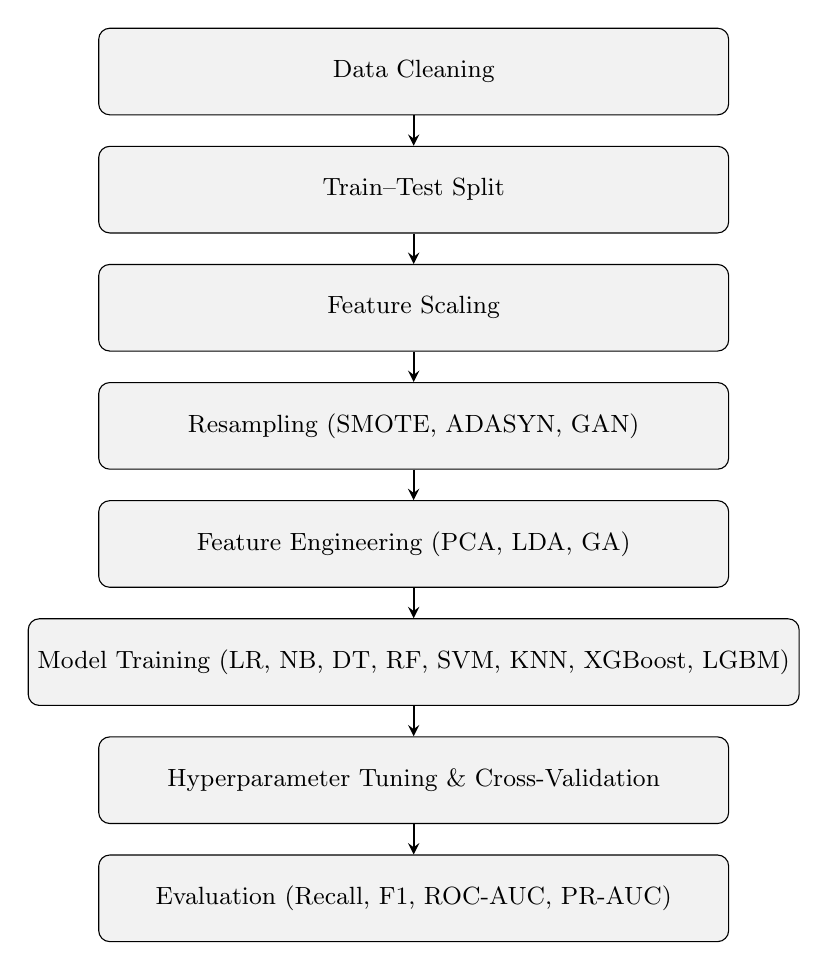
\begin{tikzpicture}[
        node distance=1.5cm,
        block/.style={
            rectangle,
            rounded corners,
            minimum width=8cm,
            minimum height=1.1cm,
            align=center,
            draw=black,
            fill=gray!10,
            font=\small
        },
        arrow/.style={thick,->,>=stealth}
    ]

    % Nodes
    \node (clean) [block] {Data Cleaning};

    \node (split) [block, below of=clean] {Train--Test Split};

    \node (scale) [block, below of=split] {Feature Scaling};

    \node (sample) [block, below of=scale] {Resampling (SMOTE, ADASYN, GAN)};

    \node (feat) [block, below of=sample] {Feature Engineering (PCA, LDA, GA)};

    \node (model) [block, below of=feat] {Model Training (LR, NB, DT, RF, SVM, KNN, XGBoost, LGBM)};

    \node (tuning) [block, below of=model] {Hyperparameter Tuning \& Cross-Validation};

    \node (eval) [block, below of=tuning] {Evaluation (Recall, F1, ROC-AUC, PR-AUC)};

    % Arrows
    \draw[arrow] (clean) -- (split);
    \draw[arrow] (split) -- (scale);
    \draw[arrow] (scale) -- (sample);
    \draw[arrow] (sample) -- (feat);
    \draw[arrow] (feat) -- (model);
    \draw[arrow] (model) -- (tuning);
    \draw[arrow] (tuning) -- (eval);

    \end{tikzpicture}

    \caption{Workflow of the Research Methodology}
    \label{fig:workflow}
\end{figure}